%THIS IS AN EXAMPLE OF HOW YOU MIGHT INTRODUCE A CHAPTER WHICH HAS ALREADY BEEN PUBLISHED.
\cleartoevenpage
\pagestyle{empty}	%Use this to suppress the header from the preceding chapter.


\begin{table}[h]
	\begin{center}
	\begin{tabular}{|c|l|l|}
		\hline
		Contributor & Statement of contribution & \% \\
		\hline
		\textbf{Edward M. Barry}	    & writing of text 			& 70\\
										& proof-reading				& 60 \\
										& theoretical derivations 	& 70 \\
										& numerical calculations 	& 100\\
										& preparation of figures 	& 100 \\
										& initial concept			& 60 \\
		\hline
		Christopher T. DeGroot			& writing of text 			& 20\\
										& proof-reading				& 10 \\
										& supervision, guidance 	& 20\\
										& theoretical derivations 	& 10\\
										& preparation of figures 	& 20 \\
										& initial concept			& 10 \\
		\hline
		Shakil Ahmmed       			& writing of text 			& 20\\
										& proof-reading				& 10 \\
										& supervision, guidance 	& 20\\
										& theoretical derivations 	& 10\\
										& preparation of figures 	& 20 \\
										& initial concept			& 10 \\
		\hline
		Tim H\"{u}lsen		    		& writing of text 			& 10\\
										& proof-reading				& 30 \\
										& supervision, guidance 	& 80 \\
										& theoretical derivations 	& 20 \\
										& preparation of figures 	& 10 \\
										& initial concept			& 80 \\
		\hline
		Damien J. Batstone	    		& writing of text 			& 10\\
										& proof-reading				& 30 \\
										& supervision, guidance 	& 80 \\
										& theoretical derivations 	& 20 \\
										& preparation of figures 	& 10 \\
										& initial concept			& 80 \\
		\hline
	\end{tabular}
	\end{center}
\end{table}


%-------------------------------------------------------------------------------------------------------%
%-------------------------------------------------------------------------------------------------------%
%-------------------------------------------------------------------------------------------------------%
%-------------------------------------------------------------------------------------------------------%
%-------------------------------------------------------------------------------------------------------%
%-------------------------------------------------------------------------------------------------------%
%This is an internal chapter of the thesis.
%If you have a long title, you can supply an abbreviated version to print in the Table of Contents using the optional argument to the \chapter command.
\chapter[A multidimensional, phototrophic, continuum biofilm model]{A multidimensional, phototrophic, continuum biofilm model}
\label{chap:ch4}	%CREATE YOUR OWN LABEL.
\pagestyle{headings}

\section*{Abstract}

%-------------------------------------------------------------------------------------------------------%
%-------------------------------------------------------------------------------------------------------%
%-------------------------------------------------------------------------------------------------------%
\section{Introduction}

%As biofilms are spatially heterogeneous structures, both spatial and temporal variations must be considered in order to describe the physical phenomena. Biofilm models can be divided into three main classes: \textit{i)} one-dimensional models capable of including mass transfer, reaction/diffusion, and detachment processes \cite{horn2014}, \textit{ii)} multidimensional discrete biofilm models such as cellular automata and agent based methods \cite{wang2010}, and \textit{iii)} continuum models including computational fluid dynamics (CFD) approaches \cite{alpkvist2007, duddu2009, cunault2015}. Despite the vast suite of modelling approaches and examples existing within the literature, there have been few studies which defining biofilm behaviour in phototrophic systems, where the spatially varying nature of the radiative field could be an important factor in the heterogeneous formation of biofilms. \\

%Representing biomass as continua can be advantageous. Firstly, the currency of process engineering modelling is differential balance equations. Continuum modelling is therefore a common language for communication of model development and results, and additionally, conservation of differential states can be ensured. In contrast to discrete modelling methods, deterministic solutions can be obtained for continuum-based models \cite{mattei2018}. Difficulties can arise when modelling continuum-based biofilms. The frequently abrupt density jumps across liquid/solid boundaries can lead to numerical instabilities. The coupling of the non-linear transport equations with growth kinetics can also be problematic. Additionally, solving state equations with vastly different time constants (and order of 10s of seconds for fluid flow in a reactor, to hours or days for biomass growth and decay expressions) can make the resolution of the time discretisation difficult. Differential algebraic equations, or appropriate time discretion algorithms for stiff systems of differential equations can overcome this barrier. Computational fluid dynamics (CFD) packages can assist with some of the numerical problems and the mathematical formulation difficulties associated with continuum models.


% \begin{itemize}
% \item Biofilms are communities of microorganisms, EPS matrices and inert substances living together
% \item There are extrinsic properties leading to their growth:
% \begin{itemize}
% \item fluid flows
% \item irradiance
% \item presence of nutrients
% \item presence or absence of other microorganisms
% \item shear rates
% \item reactor geometry and operating conditions (implicitly)
% \end{itemize}
% \end{itemize}


%Whether biofilms are desired or not, a continuum based photobiofilm model has been created in order to encapsulate the important physical conditions of systems to achieve the desired ends. 



%\begin{instructional}
%Add your text here. Use \verb|\cite| to add citation labels. Reference sections, tables, and figures using \verb|\ref|. Use \verb|\eqref| for equations. The `section' symbol $\S$ is obtained using \verb|$\S$|. Figures and other floats are added using their respective environments. Use \verb|\longtable| to split tables over page.
%\end{instructional}


%%%% PROBLEM DESCRIPTION
\newpage
\section{Problem description}
\label{S:problem_description}
The modelling approach is concerned with the description of a phototrophic biofilm system consisting of purple phototrophic bacteria (PPB). The model description for this system has been previously described \cite{Puyol2017}, however this did not account for spatial variations, and by extension, biofilm formation was not considered. The phototrophic biofilm grows attached to a surface substratum. Above the biofilm is a body of nutrient-rich liquid. Incident photons of wavelength 850 \si{\nano \metre} are irradiated from either \si{\Gamma_0} or \si{\Gamma_3} into the domain \si{\Omega}, as shown in Fig. \ref{fig:2d_above}. The initial thickness of the biofilm is \SI{50}{\micro \metre} with uniformly distributed solid species. The factor of incident irradiance is also explored, with three different irradiance levels of \SI{10}{\watt \metre ^2}, \SI{30}{\watt \metre ^2}, and \SI{100}{\watt \metre ^2} being simulated from the surface substratum. Incident irradiance in all cases is assumed uniform and diffuse across the whole boundary.


% The phototrophic biofilm (PBF) model based on purple phototrophic bacteria is an extension of the models presented previously \cite{Puyol2017} (\textbf{include my model}). Biofilm treatment extends work previously carried out by \cite{alpkvist2007}, \cite{alpkvist2007}. The important physical processes identified are as follows:
% \begin{itemize}
%     \item Coupled volume of fluid and level set for capturing of the biofilm/liquid interface.
%     \item Radiative transfer coupled to the growth of the biokinetics.
%     \item Biokinetics equations coupled to the radiative transfer equation (RTE) and the biofilm advection terms.
%     \item Development of a biofilm front velocity based on the evolution of pressure due to solid species growth within the biofilm.
% \end{itemize}




\begin{figure}[htpb]
    \centering
    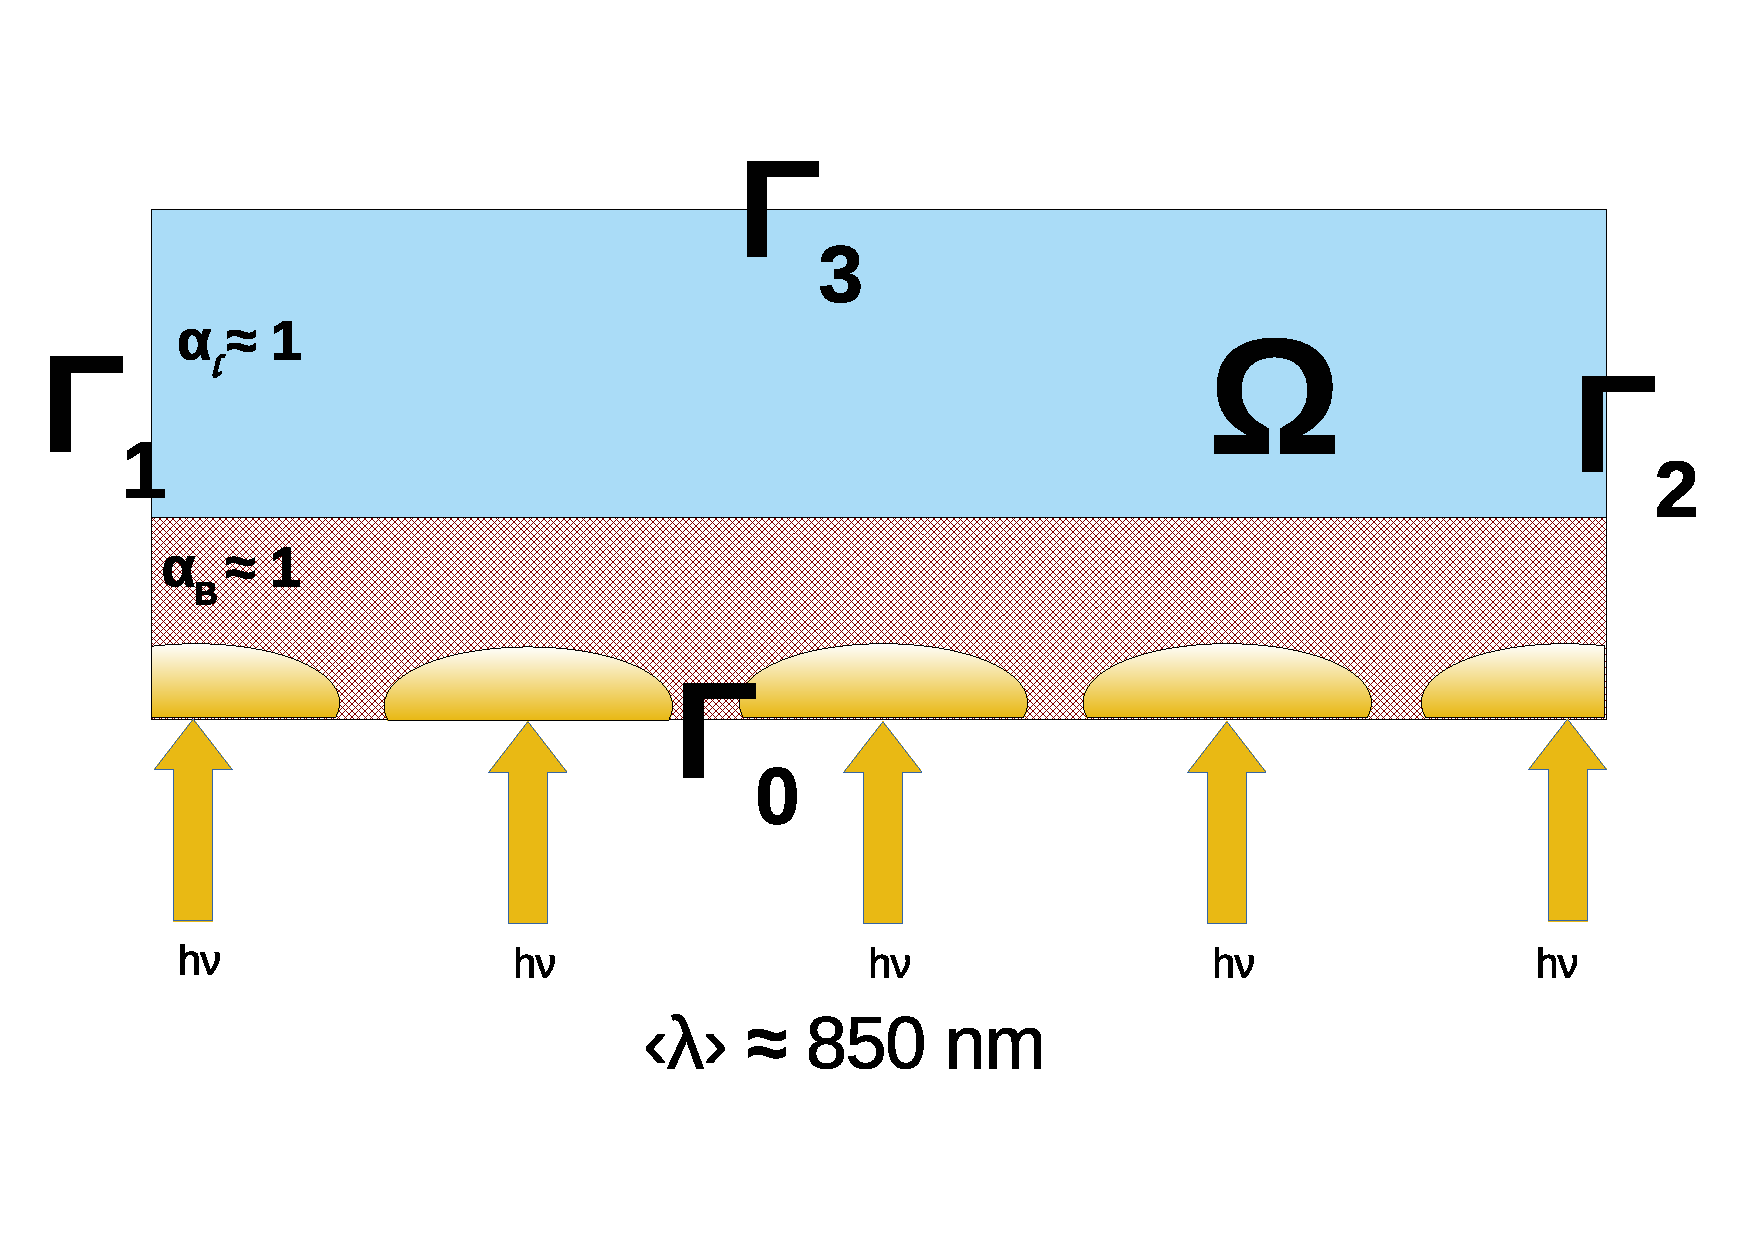
\includegraphics[scale=0.5]{Images/Chap4/prob_diagram_below.pdf}
    \caption{Two-dimensional representation of the simulation domain for the case of a bottom-irradiated biofilm. Boundaries \si{\Gamma_4} and \si{\Gamma_5} are out of, and into the page respectively, and take the same boundary conditions as boundaries \si{\Gamma_1} and \si{\Gamma_2}. The irradiance source (\si{h \nu}) is in fact uniform and diffuse across the whole boundary. Subscripts relating to \si{\alpha}, namely \textbf{l} and \textbf{B} correspond to liquid phase fraction, and biofilm phase fraction respectively.} 
    \label{fig:2d_above}
\end{figure}


%%%%%%%%%%%%% MATHEMATICAL FORMULATION

\newpage
\section{Mathematical formulation}
\label{S:formulation}
\subsection{Radiative transfer}
The general form of the radiative transfer equation (RTE) has been adapted to phototrophic systems \textbf{cite me} \cite{Kong2014}, and includes the dependency on the concentration of solid species and water. The black body radiation term has been omitted from this equation due to minimal influence on the system energy balance (Eq. \ref{eq:rteSimplified}). 

\begin{equation}
\frac{dI_\lambda (\textbf{r}, \textbf{s})}{ds} \, = \, - \sum_{j} [E_{\lambda,j} X_j] I_\lambda (\textbf{r}, \textbf{s})\, +\, \frac{\sigma_{\lambda, s, j}}{4 \pi} \int_{4 \pi} I_\lambda (\textbf{r}, \textbf{s}^\prime) \Phi_\lambda(\textbf{s}, \textbf{s}^\prime) d\Omega^\prime
    \end{equation}

where $I_\lambda$ is the spectral irradiance for a given wavelength, \textbf{r} is the position vector of a radiative ray, \textbf{s} is the direction vector of the ray, and s is the path length. The first term on the right hand side is the extinction term, with $E_{\lambda, j}$ being the specific extinction coefficient (the combination of scattering and absorption components) for participating species $X_j$. The second term on the right hand side is associated with in-scattering, where $\sigma_{\lambda, s, j}$ is the scattering coefficient, and $\Phi_\lambda$ is the wavelength scattering function from path \textbf{s} to scattered direction $\textbf{s}^\prime$ through solid angle $d\Omega$. The phase scattering function, $\Phi_\lambda$ for this model is the Schlick function (Eq. \ref{eq:schlick}), which is appropriate for optically thick media \cite{Jarosz2008}. 

\begin{equation}
\Phi_s(k, \theta) = \frac{1 \, -\,  k^2}{4\pi (1\, +\,k\, cos(\theta))^2 }
\end{equation}

where parameter $k$ takes values between -1.0 and 1.0 included, with negative or positive values corresponding to back-scattering and forward scattering respectively. A value of 0 means scattering is isotropic. The parameter $k$ represents the average cosine of the scattered angles. The angle $\theta$ is that made by the previous path and scattered path of a ray.

\subsection{Consumption and release of soluble substrates}
Soluble substrates exist in both the volume of liquid, and the biofilm volume. Their growth and release expressions (hydrolysis of biodegradable particulate organic matter) have been previously described \cite{Puyol2017}. The soluble substrates considered in this study are readily biodegradable soluble organics expressed in chemical oxygen demand (COD), acetic acid (COD), hydrogen (COD), inorganic carbon (C), inorganic nitrogen (N), inorganic phosphorus (P) and soluble inert material (COD). The general form for the soluble balance equation is expressed in Eq. \ref{eq:solubles}.

\begin{equation}
\label{eq:solubles}
\frac{\partial S_i}{\partial t} = \mathcal{D}_i\nabla^2 S_i + r_{i}
\end{equation}

where $S_i$ is the soluble species $i$, $\mathcal{D}_i$ is the diffusion coefficient of species $i$, and $r_i$ is the corresponding consumption/release equation \cite{Puyol2017}.

The transport equations for the soluble and particulate species may be written as follows,
\begin{equation}
\label{eq:solublesD}
\frac{\partial S_{\Phi}}{\partial t} + \nabla (\phi S_{\Phi}) - \nabla \cdot (D_{\Phi} \nabla S_{\Phi}) = \Gamma_{\Phi}, 
\end{equation}
\begin{equation}
\label{eq:particulate}
\frac{\partial X_{\Phi}}{\partial t} + \nabla (\phi X_{\Phi}) - \nabla \cdot (D_{\Phi} \nabla X_{\Phi}) = \Gamma_{\Phi}, 
\end{equation}
where, S is the soluble species and $\mathrm{\Phi}$ = SI, SH$\mathrm{_2}$, SIC, SAC, SIN, SIP and SS; X is the particulate species and $\mathrm{\Phi}$ = XPB, XS and XI; $\mathrm{D_{\Phi}}$, and $\mathrm{\Gamma_{\Phi}}$ are the diffusivity, and growth rate of species $\mathrm{\Phi}$, respectively.  


\subsection{Growth of particulate matter}
The growth of particulate matter forms the biofilm structure and influences the pressure equation which influences advection of the biofilm front. The particulate species included in this study are PPB, slowly biodegradable particulate organics, and inert particulate organic matter. Similarly to \cite{alpkvist2007}, replace $X_i$, the concentration of particulate species $i$ with $\rho^*\theta_i$ where $\rho^*$ is the density of particulate species, assumed constant for each species, and $\theta_i$ is the volume fraction of species $i$. The growth terms for the particulate balance equations (Eq.~\ref{eq:particulates}) have been previously defined \cite{Puyol2017}.


\begin{equation}
    \label{eq:particulates}
    \frac{\partial \theta_i}{\partial t} = \lambda \nabla p \cdot \nabla \theta_i + \frac{g_i}{\rho^*} - \theta_i \sum_{i=1}^{N_{\theta_i}}\frac{g_i}{\rho^*}
\end{equation}

where 

\subsection{Hydrodynamics}
\label{Hydro}
The multiphase flow may be calculated employing the mixture mass, momentum and continuity equations as follows,

\begin{equation}
    \label{eq:continuity}
    \nabla \cdot U = \Gamma,
\end{equation}

\begin{equation}
    \label{eq:mass}
    \frac{\partial \alpha}{\partial t} + \nabla\cdot (\phi \alpha) = \Dot{m},
\end{equation}

\begin{equation}
    \label{eq:momentum}
    \frac{\partial (\rho U)}{\partial t} + \nabla\cdot (\rho U U) = -\nabla P + \rho g+\nabla \cdot (\tau+\tau_t)+f_{\sigma},
\end{equation}
where, U is the velocity, $\mathrm{\Gamma}$ is the growth term, $\mathrm{\alpha}$ is the phase fraction, $\mathrm{\phi}$ is the mass flux, $\mathrm{\Dot{m}}$ is the mass transfer, $\mathrm{\rho}$ is the density, g is the gravitational acceleration, P is the pressure, $\mathrm{\tau}$ is the viscous stress, $\mathrm{\tau_t}$ is the turbulent stress, and $\mathrm{f_{\sigma}}$ is the surface tension force. As the mixture method, the density $\mathrm{\rho}$ is expressed as the mixture density as,  

\begin{equation}
    \label{eq:mixtureDensity}
    \rho = \rho_1 \alpha + \rho_2 (1-\alpha),
\end{equation}
where, $\mathrm{\rho_1}$ and $\mathrm{\rho_2}$ are the densities of the phase one and phase two, respectively. The surface tension force $\mathrm{f_{\sigma}}$ may be calculated as follows,
\begin{equation}
    \label{eq:surfaceTension}
    f_{\sigma} = \sigma k \nabla\alpha.
\end{equation}
Here, $\mathrm{\sigma}$, and $k$ are the surface tension coefficient, and curvature, respectively. The curvature $k$ may be written as, 

\begin{equation}
    \label{eq:curvature}
    k = -\nabla \mathbf{n} = -\nabla \Bigg(\frac{\nabla \alpha}{\big| \nabla \alpha\big|} \Bigg),
\end{equation}
where, \textbf{n} is the outward unit normal vector at the interface.

\subsection{Operating parameters and model assumptions}


\section{Applications}
\subsection{Boundary and initial conditions}
A series of six operating conditions were simulated in order to highlight the important aspects of the model. These cases were selected because previous studies had noted that radiation delivery and readily biodegradable soluble organics were the major limitations to reactor performance in a suspended growth context \cite{Hulsen2016, Hulsen2016a}. The rationale was thus that simulations exploring these limitations would aid in understanding the dynamics of phototrophic biofilm growth. In the base cases, the radiative intensity was delivered from below an assumed transparent substratum. In addition to the limiting concentrations and intensities of acetate and radiation, different configurations were explored. Firstly, the baseline experiment with both radiative intensity and acetate in sufficient quantities was repeated with the radiation source from above the biofilm. Finally, the above/below incident irradiances were repeated with a substratum initially sparsely populated with phototrophic biofilm (summarised in Table \ref{tab:biofilm_cases}). 

\begin{table}[H]
    \centering
    \small
    \renewcommand{\arraystretch}{1.4}
    \caption{Suite of differing operating conditions for the biofilm simulations for both 2D and 3D cases.}
    \tabcolsep=0.11cm
    \begin{tabular}{@{}p{1cm} p{2cm} p{3cm} p{5cm} p{5cm}@{}} \toprule
Case & Irradiance  & S\textsubscript{AC\textsubscript{0}}  & \{$\alpha$\textsubscript{PB\textsubscript{0}}, $\alpha$\textsubscript{S\textsubscript{0}}, $\alpha$\textsubscript{I\textsubscript{0}}\}  &  Configuration \\ \hline
1    &  30 Wm\textsuperscript{-2}  &    0.8 kg COD m\textsuperscript{-3}    &  \{0.5, 0.4, 0.1\}$\mathds{1}^*_{y<0.03mm}$  & Incident below\\
2     &  30 Wm\textsuperscript{-2}  &    0.2 kg COD m\textsuperscript{-3}    &  \{0.5, 0.4, 0.1\}$\mathds{1}_{y<0.03mm}$ & Incident below\\
3    &  5 Wm\textsuperscript{-2}  &    0.8 kg COD m\textsuperscript{-3}    &  \{0.5, 0.4, 0.1\}$\mathds{1}_{y<0.03mm}$  & Incident below\\
4    &  30 Wm\textsuperscript{-2}  &    0.8 kg COD m\textsuperscript{-3}    &  \{0.5, 0.4, 0.1\}$\mathds{1}_{y<0.03mm}$  & Incident above\\
5    &  30 Wm\textsuperscript{-2}  &    0.8 kg COD m\textsuperscript{-3}    &  \{0.5, 0.4, 0.1\}  & Sparse biofilm, incident below\\
6    &  30 Wm\textsuperscript{-2}  &    0.8 kg COD m\textsuperscript{-3}    &  \{0.5, 0.4, 0.1\}  & Sparse biofilm, incident above\\ \hline
    \end{tabular}
  \scriptsize{
     * $\mathds{1}$ is the characteristic function where the stated initial biofilm concentration applies if the condition is true, or is zero if false.} 
    \label{tab:biofilm_cases}
\end{table}

For all other state variables, initial and boundary conditions were maintained constant across all simulations.\\

In the case of boundary conditions, the velocity field was treated as the no-slip at the boundaries whereas the fixed-flux-pressure was imposed for the pressure field. Conversely, in the case of phase fractions, i.e. $\mathrm{\alpha}$, the inlet-outlet boundary condition, which is a mixture of zero-gradient and fixed-value boundary conditions, is considered at the outlet, and the walls are treated as zero-gradient. The boundary conditions may be summarised as,  

\begin{equation}
    \label{eq:boundaryU}
    U_x = U_y = U_z = 0, \quad \mathrm{at \, walls\, and\, outlet},
\end{equation}

\begin{equation}
    \label{eq:boundaryPrgh}
    \nabla P_{rgh} = \bigg[\frac{\phi \frac{H(U)}{a_p} - \phi}{|S_f|a_p} \bigg], \quad \mathrm{at \, walls\, and\, outlet},
\end{equation}

\begin{equation}
    \label{eq:boundaryAlpha}
    \frac{\partial \alpha}{\partial n} = 0 \quad \mathrm{and} \quad \alpha = \alpha_i \quad \mathrm{at \, walls\, and\, outlet}.
\end{equation}

Here, $\mathrm{P_{rgh}}$ is the pressure less the hydrostatic head, and H(U), $\mathrm{a_P}$, $\mathrm{\phi}$, and $\mathrm{S_f}$ are the transported coefficients, matrix coefficients related to the variables, such as U, flux, and surface area vector, respectively, of the discretised governing equations; n = x = y = z, and $\mathrm{\alpha_i}$ is the internal cell centre value close to the boundary face. The initial conditions for the velocity and pressure fields are set zero. The volume phase fractions are initialised by defining the values for $\alpha_{\mathrm{XPB}}$, $\alpha_{\mathrm{XS}}$, $\alpha_{\mathrm{XS}}$, and $\alpha_{\mathrm{w}}$. The volume fractions were set such that their sum was unity for all cells within the domain. 


%%%%%%%%%%%%%%%%% Implementation
\section{Implementation}

\subsection{Case 5: Sparsely initiated biofilm irradiated from substratum}
\begin{figure}[H]
    \centering
    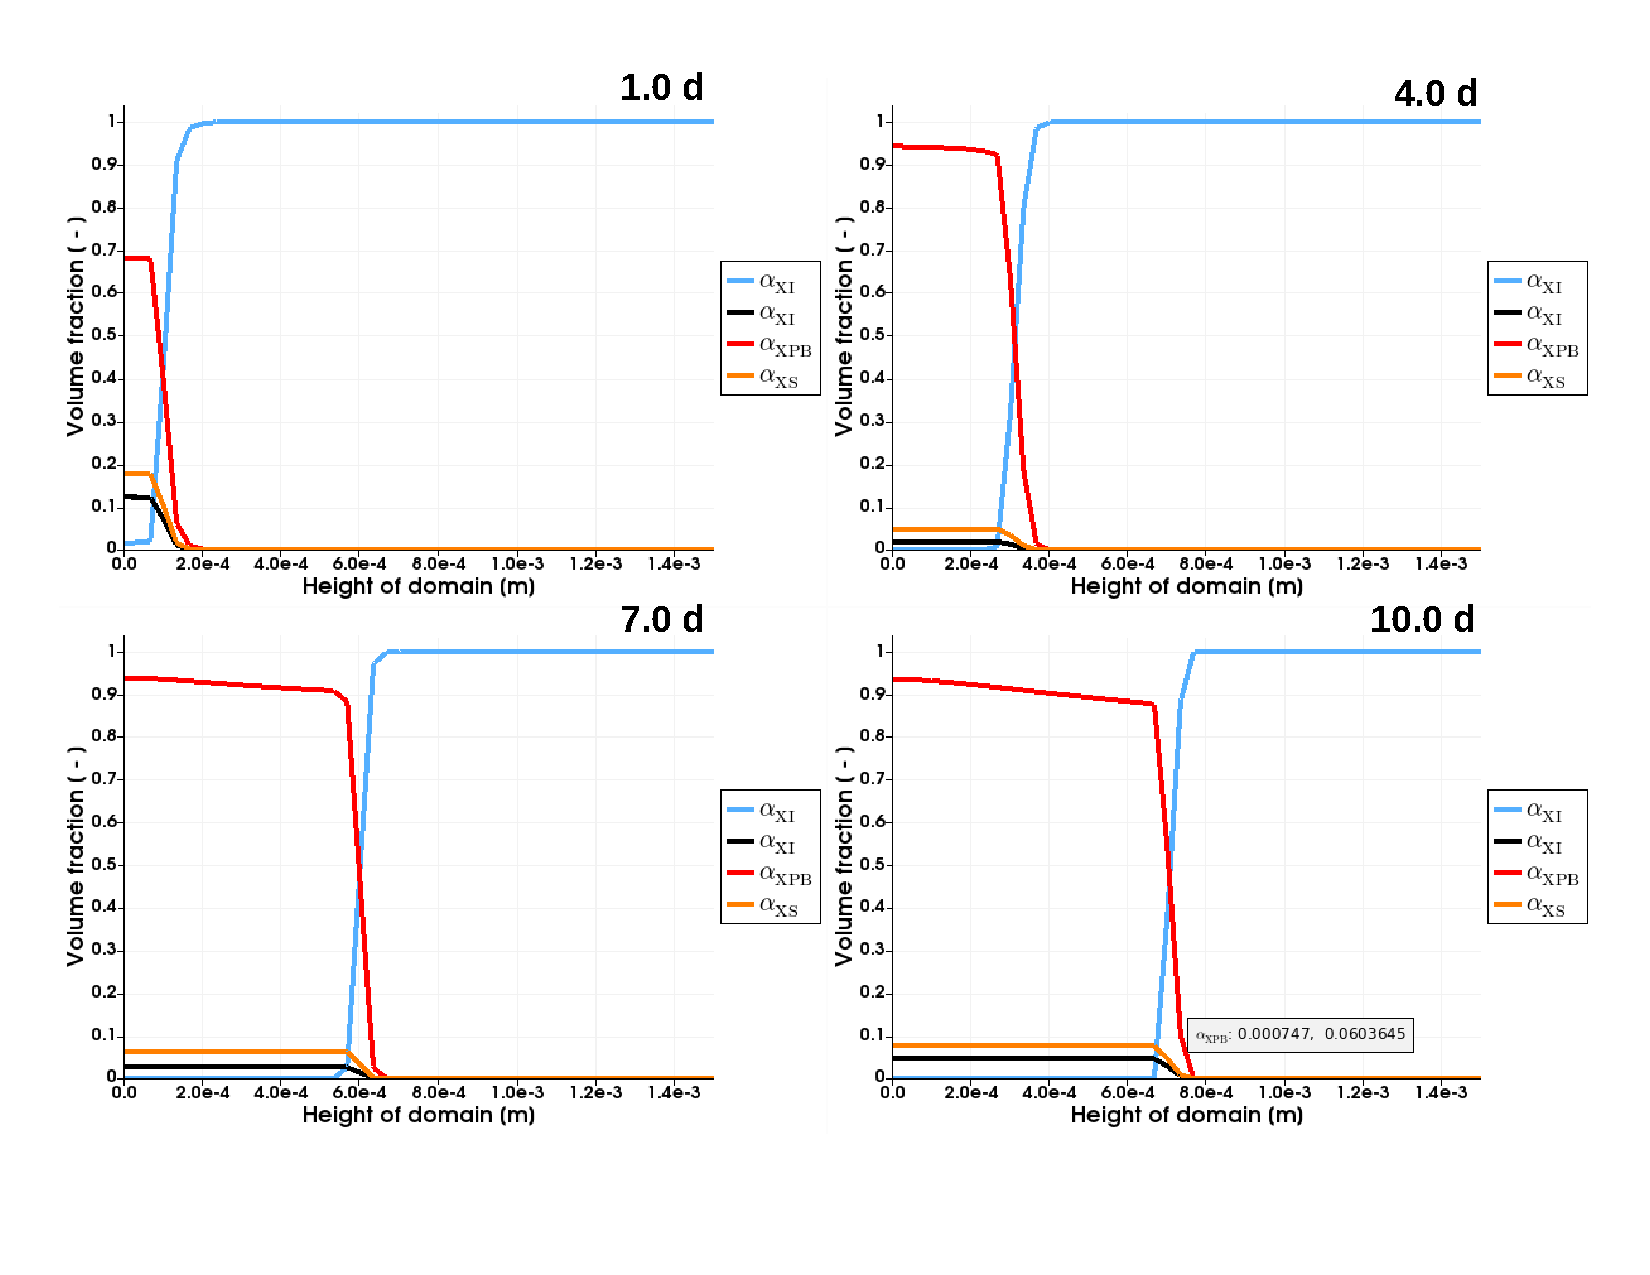
\includegraphics[width=\textwidth,height=0.5\textheight]{Chap4/results/post_processing/renders/case5_3D/case5_3D_dist.pdf}
    \caption{Three dimensional render of PPB growth as biofilm over a substratum irradiated at 30 W m\textsuperscript{-2} at 850 nm. } 
    \label{fig:case5_alpha_distro}
\end{figure}


\begin{figure}[tp]
    \centering
    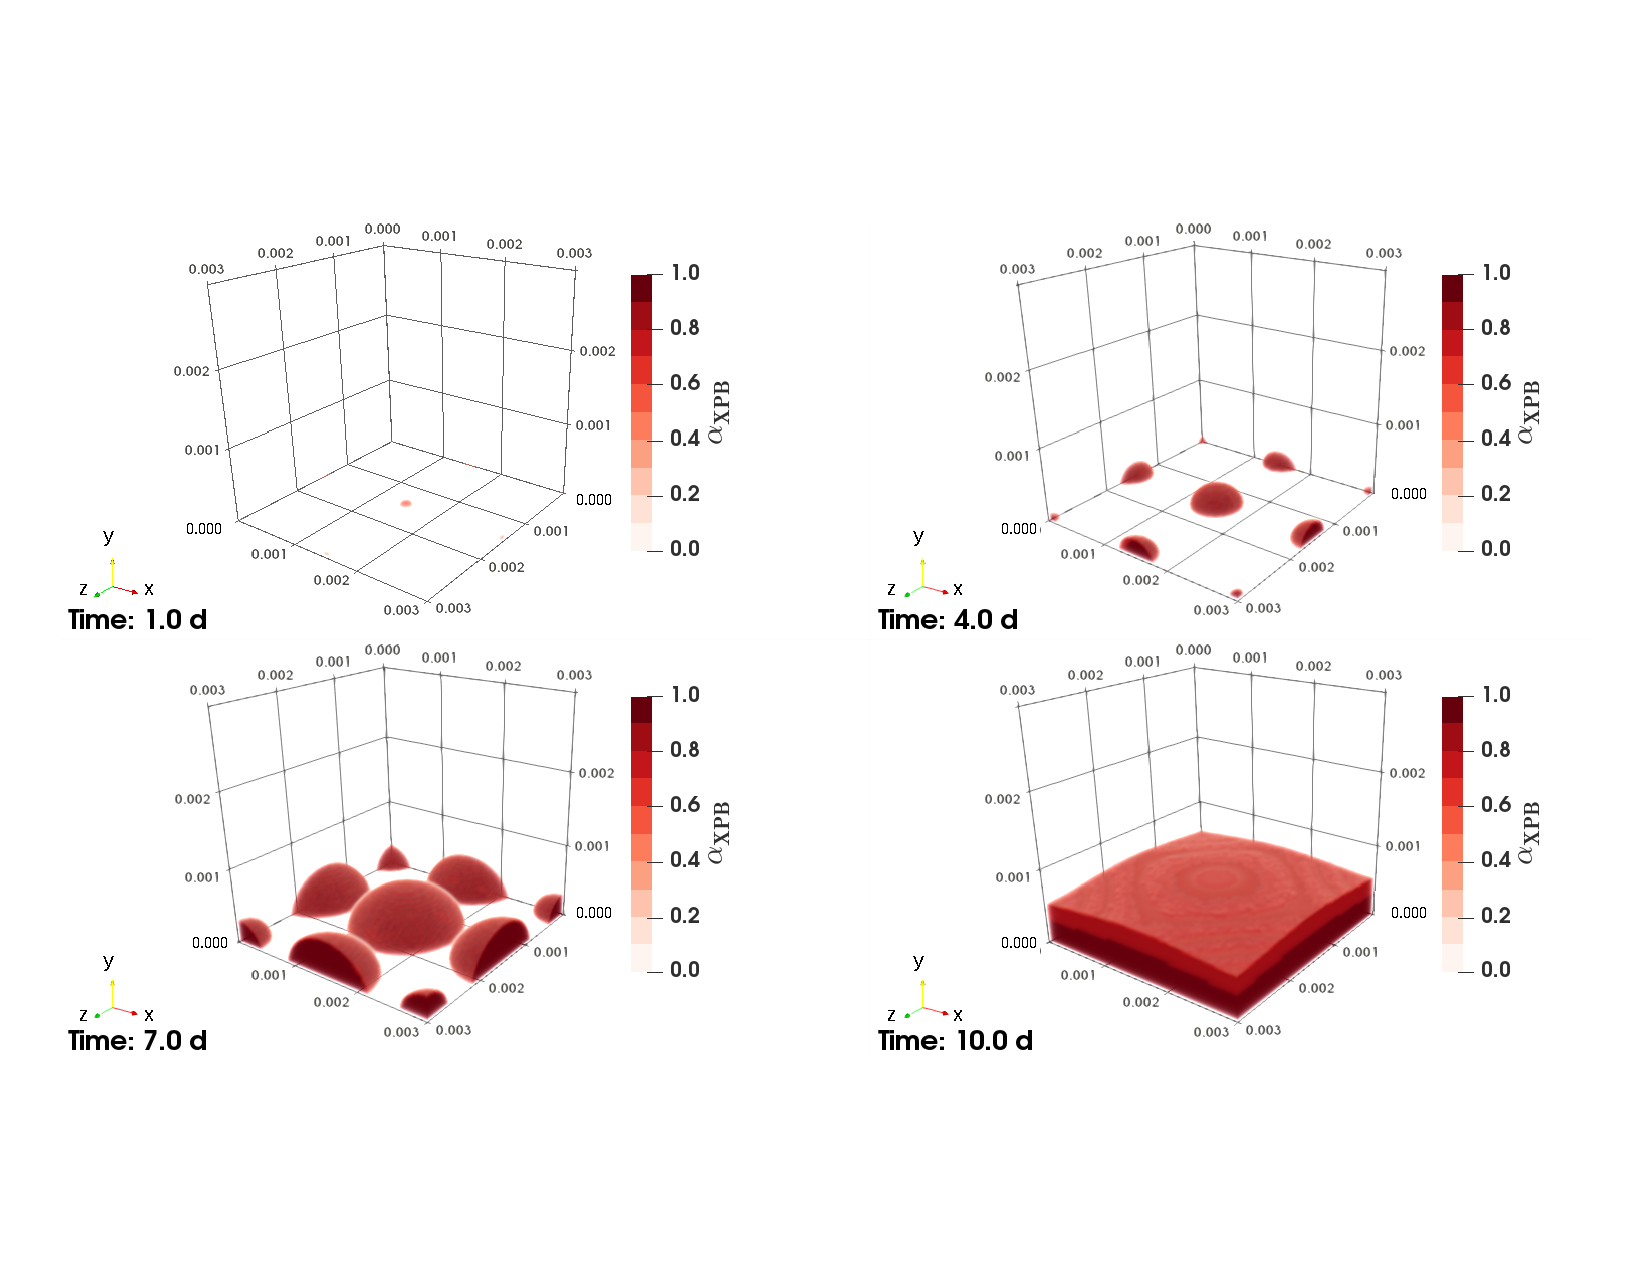
\includegraphics[width=\textwidth,height=0.5\textheight]{Chap4/results/post_processing/renders/case5_3D/case5_3D_ppb.pdf}
    \caption{Three dimensional render of PPB growth as biofilm over a substratum irradiated at 30 W m\textsuperscript{-2} at 850 nm. } 
    \label{fig:case5_3D_ppb}
\end{figure}


\begin{figure}[tp]
    \centering
    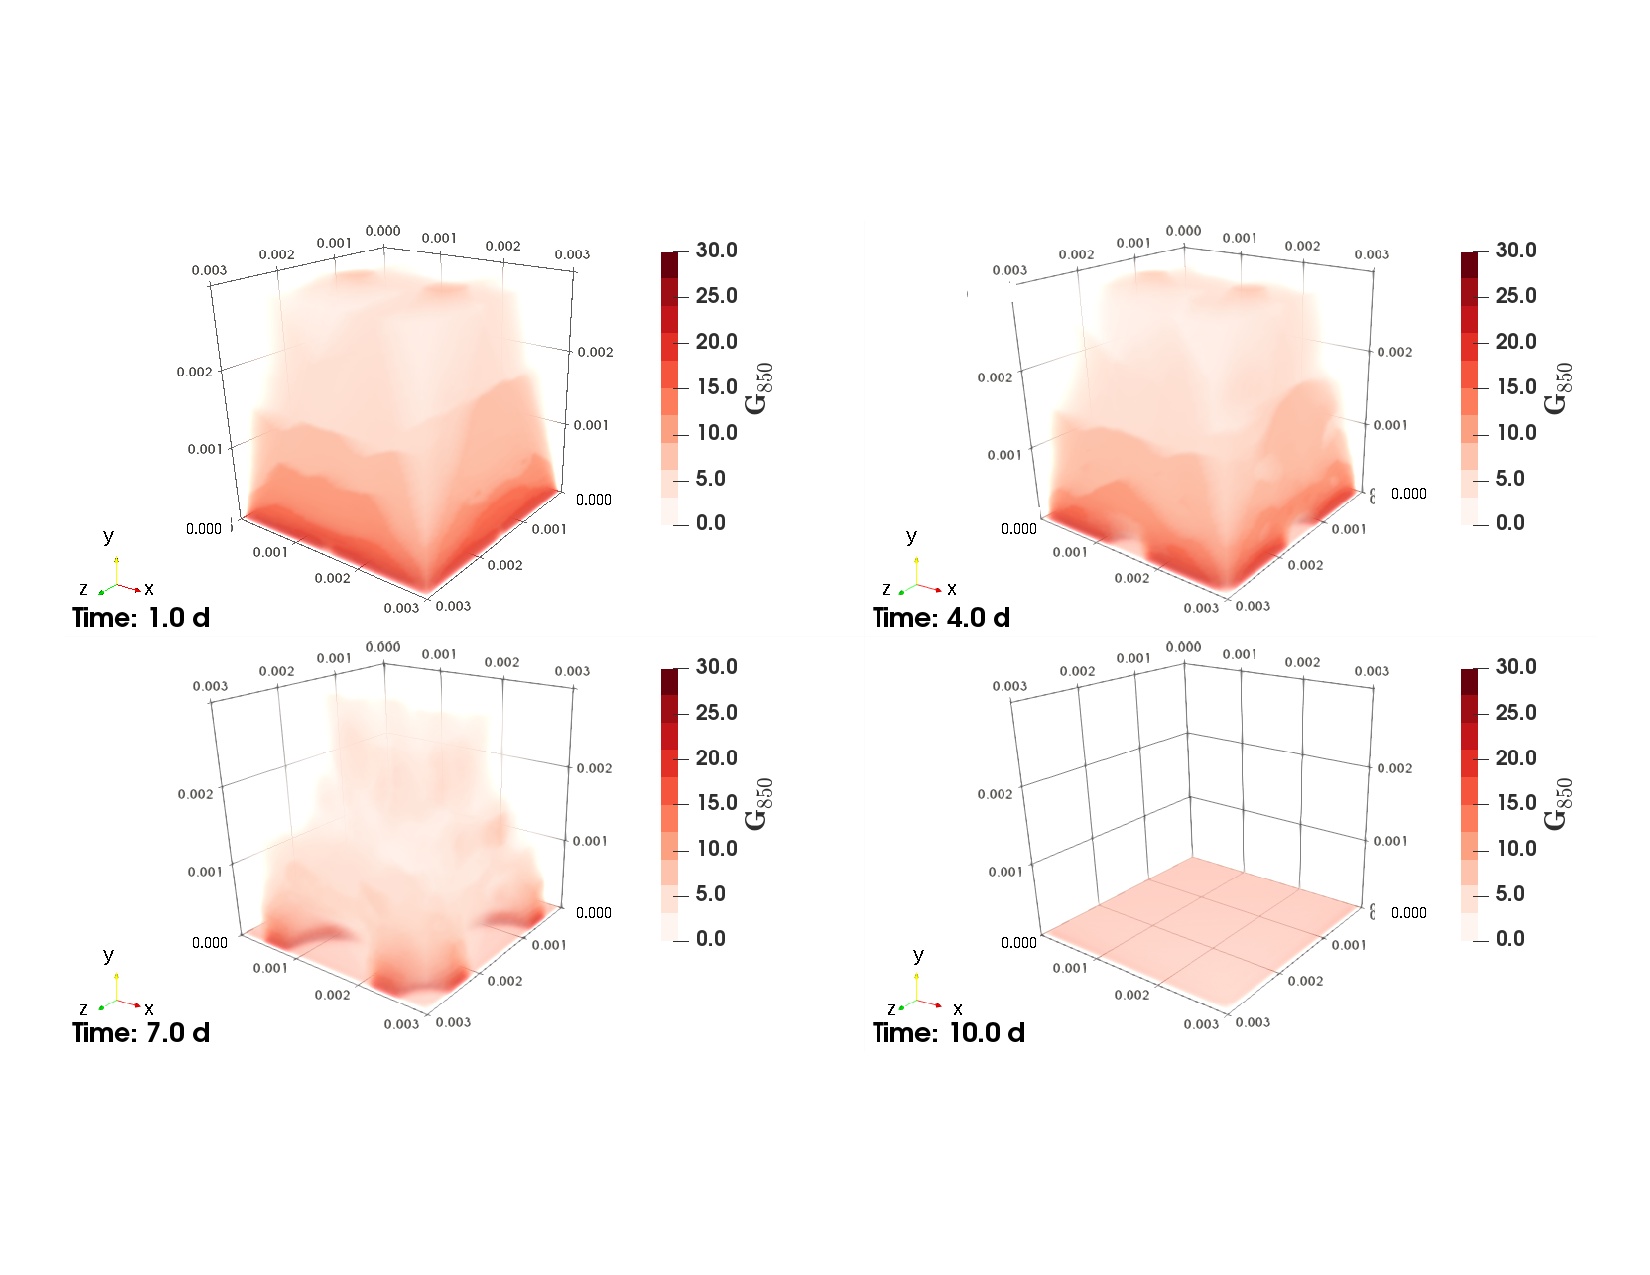
\includegraphics[width=\textwidth,height=0.5\textheight]{Chap4/results/post_processing/renders/case5_3D/case5_3D_rad.pdf}
    \caption{Three dimensional render of PPB growth as biofilm over a substratum irradiated at 30 W m\textsuperscript{-2} at 850 nm. } 
    \label{fig:case5_3D_rad}
\end{figure}



\subsection{Case 6: Sparsely distributed biofilm irradiated from above}

\begin{figure}[tp]
    \centering
    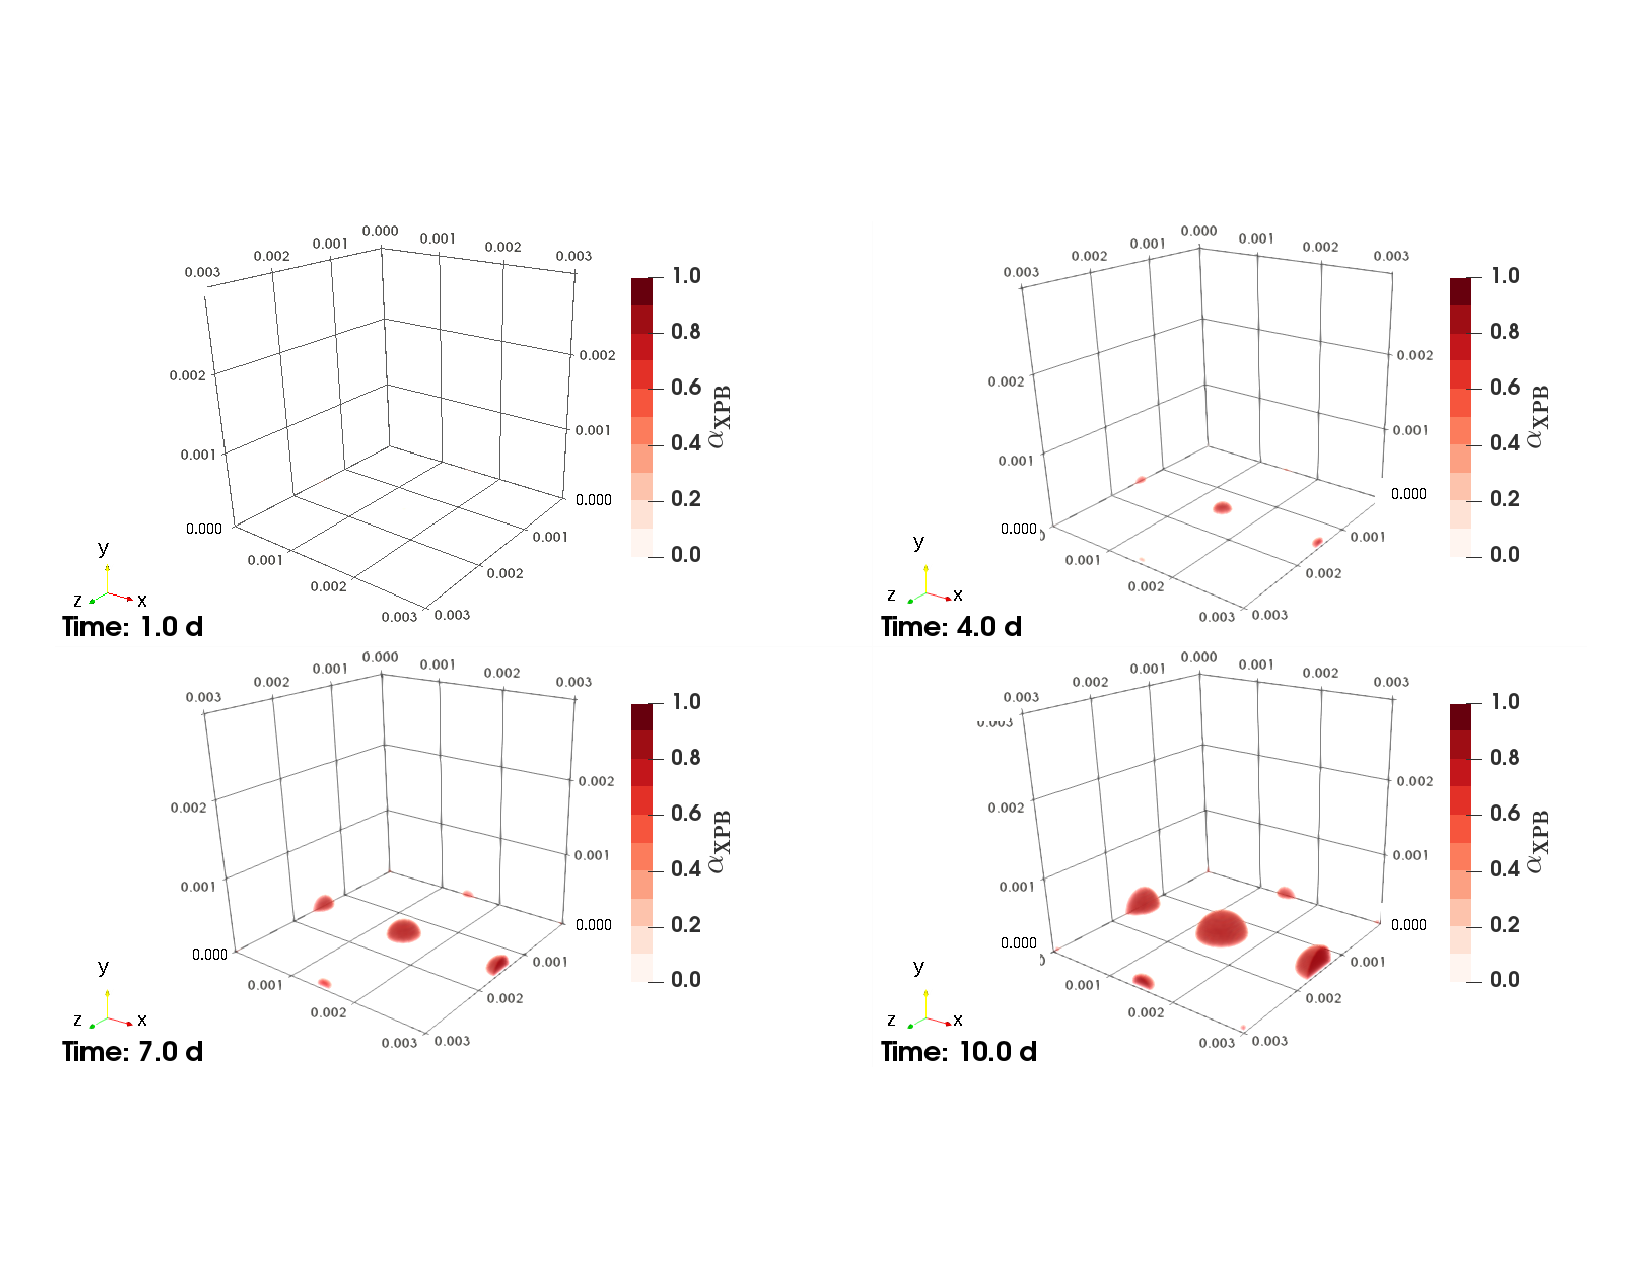
\includegraphics[width=\textwidth,height=0.4\textheight]{Chap4/results/post_processing/renders/case6_3D/case6_3D_dist.pdf}
    \caption{Three dimensional render of PPB growth as biofilm over a substratum irradiated at 30 W m\textsuperscript{-2} at 850 nm. } 
    \label{fig:case6_3D_dist}
\end{figure}

\begin{figure}[tp]
    \centering
    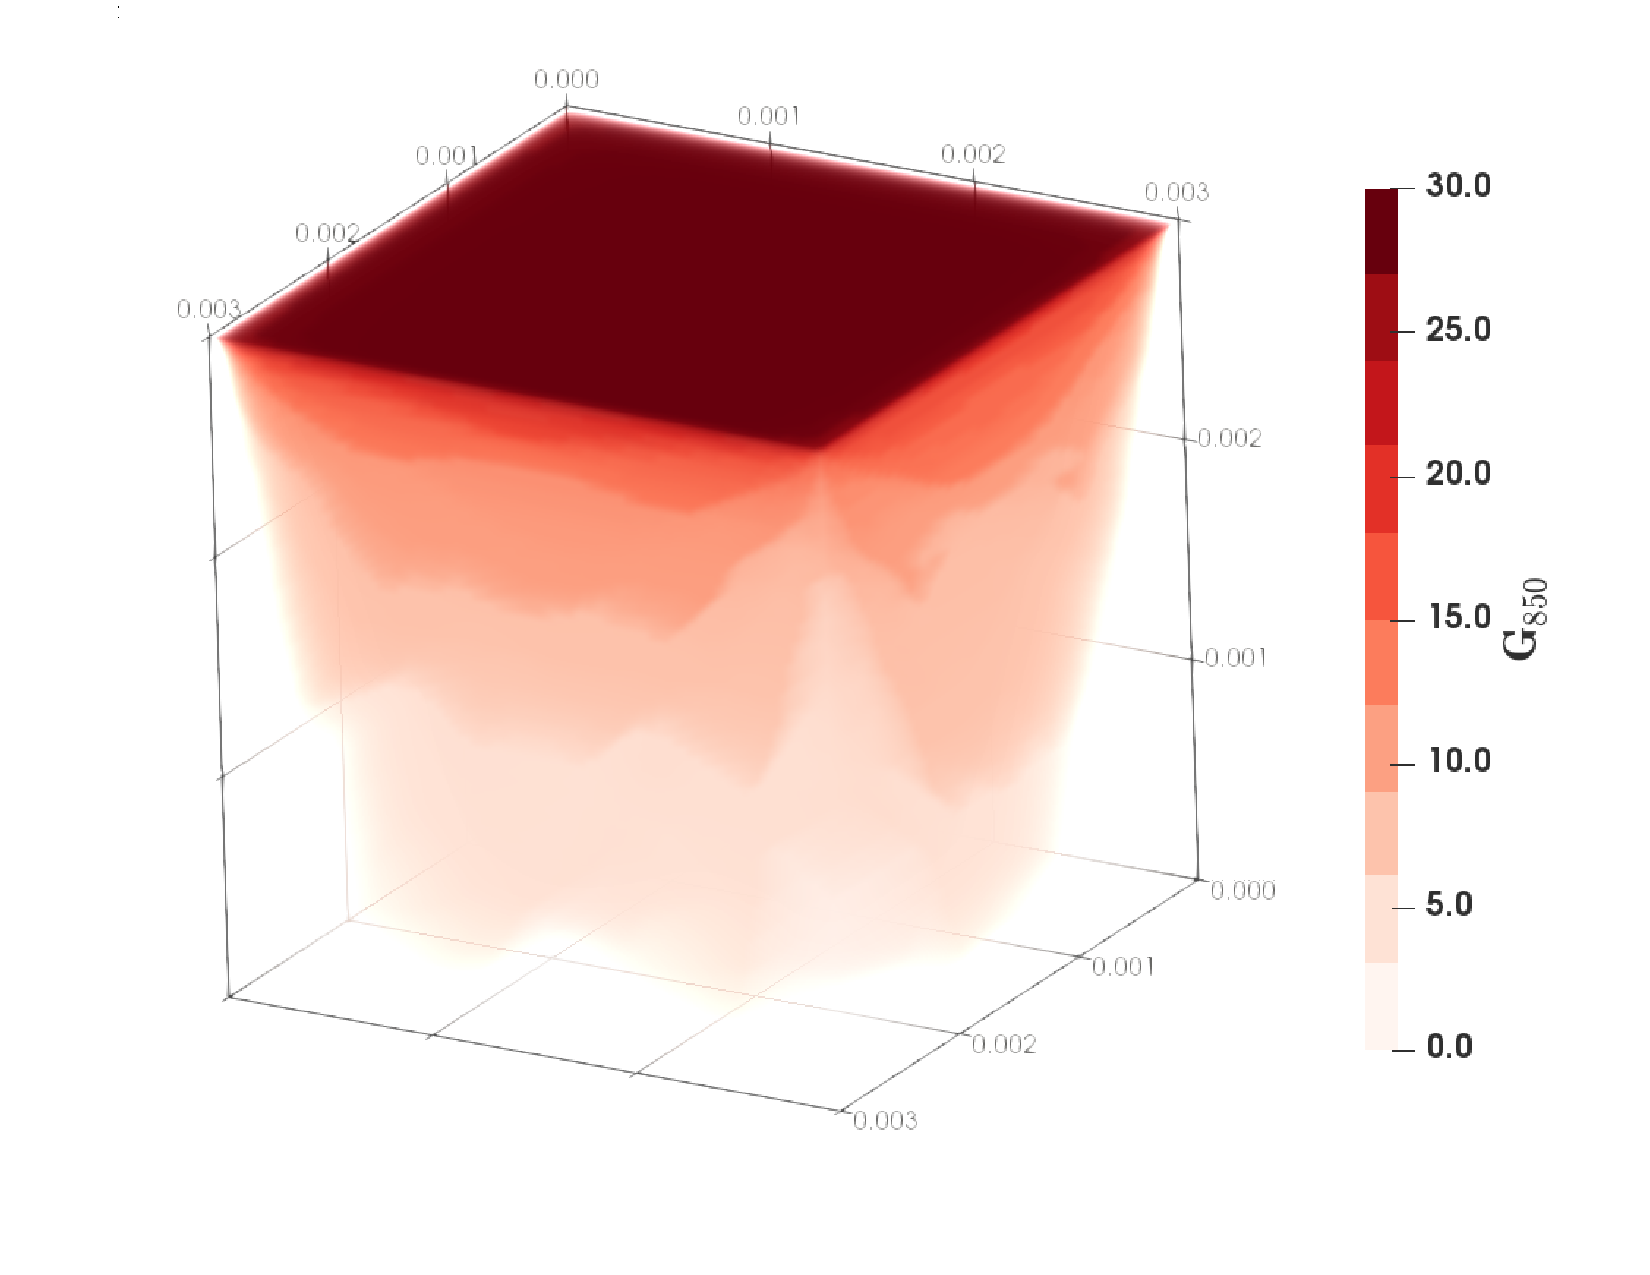
\includegraphics[width=\textwidth,height=0.5\textheight]{Chap4/results/post_processing/renders/case6_3D/case6_3D_rad.pdf}
    \caption{Three dimensional render of PPB growth as biofilm over a substratum irradiated at 30 W m\textsuperscript{-2} at 850 nm. } 
    \label{fig:case6_3D_rad}
\end{figure}

\begin{figure}[tp]
    \centering
    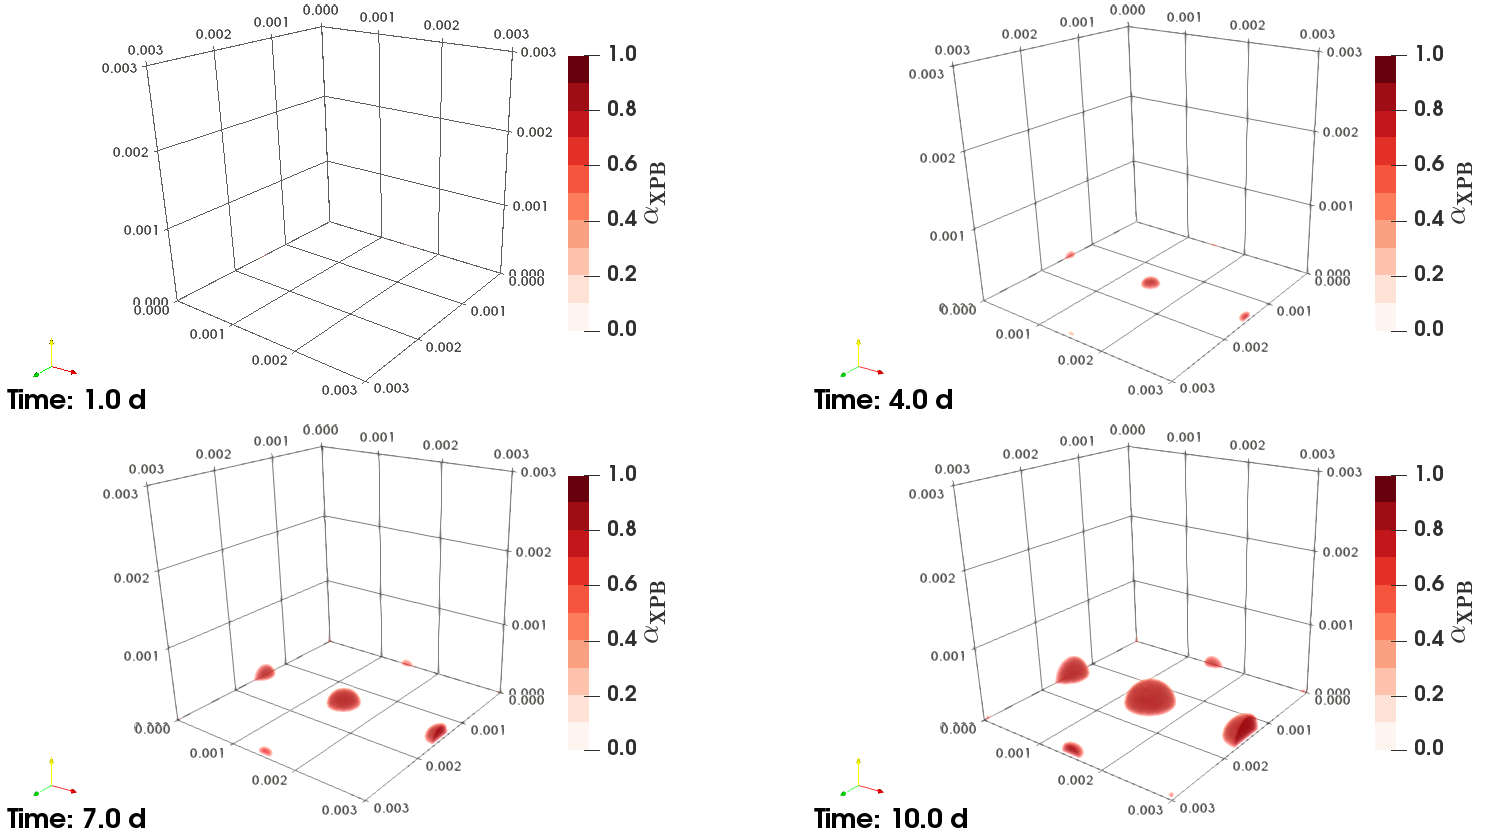
\includegraphics[width=\textwidth,height=0.5\textheight]{Chap4/results/post_processing/renders/case6_3D/case6_ppb_3D.png}
    \caption{Three dimensional render of PPB growth as biofilm over a substratum irradiated at 30 W m\textsuperscript{-2} at 850 nm. } 
    \label{fig:case6_3D_ppb}
\end{figure}










%%%%%%%%%%%%%%%%%%%%%%%% DISCUSSION
\section{Discussion}

\begin{figure}[tp]
    \centering
    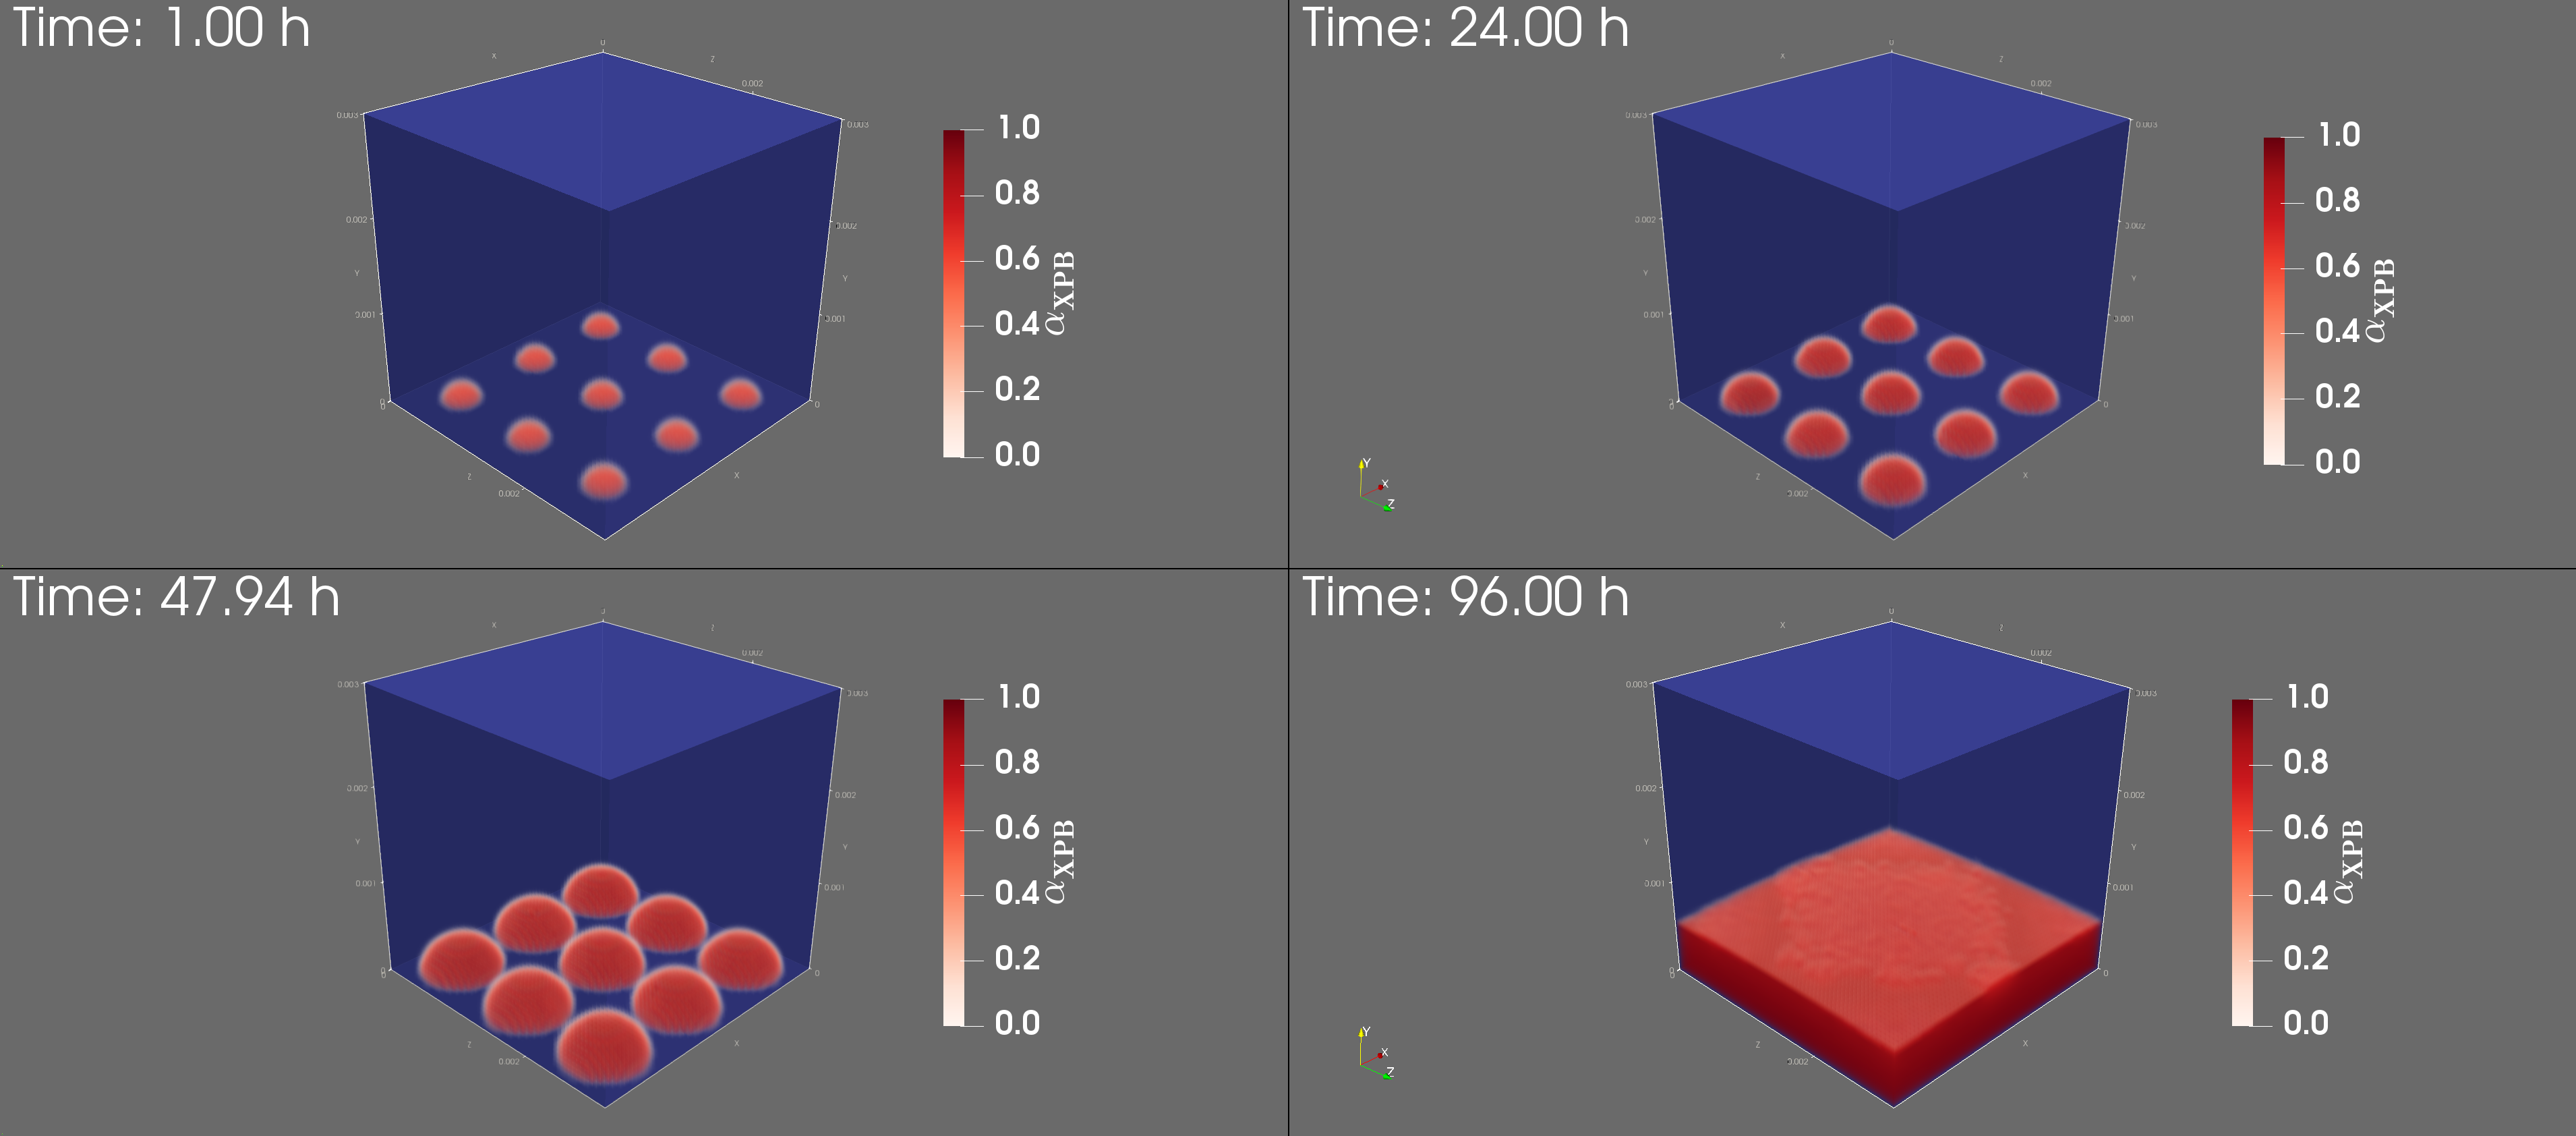
\includegraphics[width=\textwidth,height=0.4\textheight]{Chap4/results/xpb_alpha_volumeRender.png}
    \caption{Three dimensional render of PPB growth as biofilm over a substratum irradiated at 30 W m\textsuperscript{-2} at 850 nm. } 
    \label{fig:3d_below_ppb}
\end{figure}




\begin{figure}[tp]
    \centering
    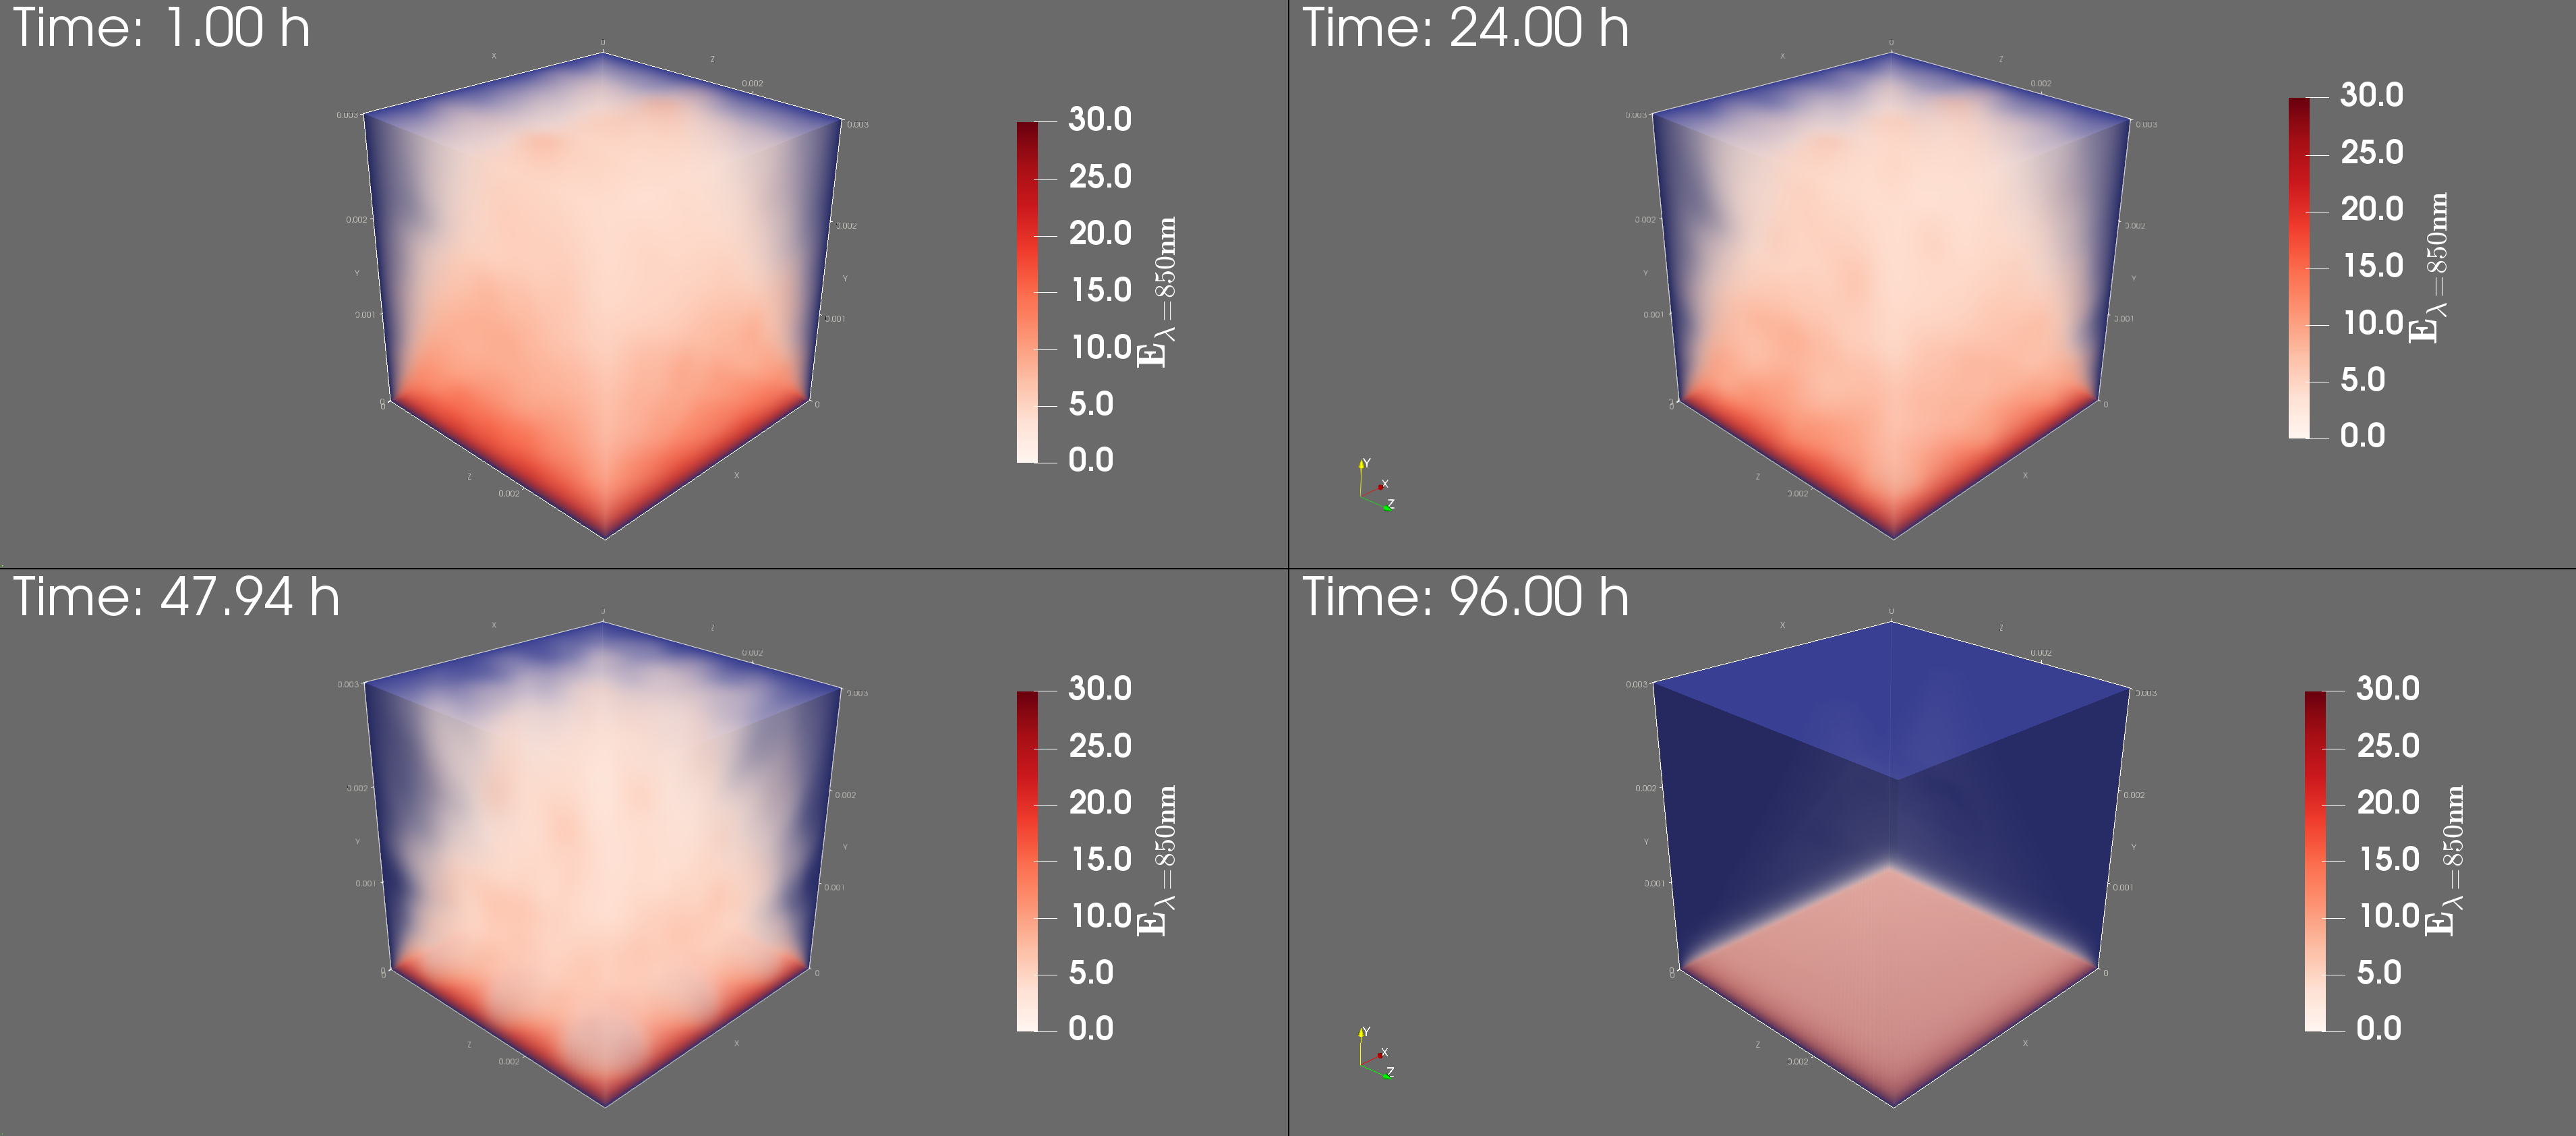
\includegraphics[width=\textwidth,height=0.4\textheight]{Chap4/results/E850_below_3d.png}
    \caption{Three dimensional render of the radiative field as biomass grows in time. The incident irradiance is set from the substratum at 30 W m\textsuperscript{-2}. } 
    \label{fig:3d_below_rad}
\end{figure}












%%%%%%%%%%%%%%%%%%% CONCLUSIONS
\section{Conclusions}